\begin{center}
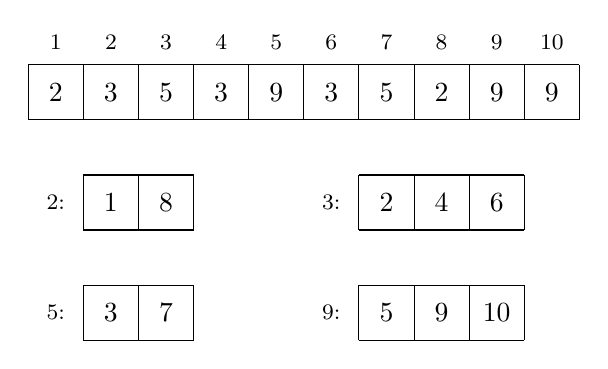
\begin{tikzpicture}[scale=0.7]
\draw (0,0) grid (10,1);

\node at (0.5,0.5) {$2$};
\node at (1.5,0.5) {$3$};
\node at (2.5,0.5) {$5$};
\node at (3.5,0.5) {$3$};
\node at (4.5,0.5) {$9$};
\node at (5.5,0.5) {$3$};
\node at (6.5,0.5) {$5$};
\node at (7.5,0.5) {$2$};
\node at (8.5,0.5) {$9$};
\node at (9.5,0.5) {$9$};

\footnotesize
\node at (0.5,1.4) {$1$};
\node at (1.5,1.4) {$2$};
\node at (2.5,1.4) {$3$};
\node at (3.5,1.4) {$4$};
\node at (4.5,1.4) {$5$};
\node at (5.5,1.4) {$6$};
\node at (6.5,1.4) {$7$};
\node at (7.5,1.4) {$8$};
\node at (8.5,1.4) {$9$};
\node at (9.5,1.4) {$10$};

\normalsize
\draw (1,-1) grid (3, -2);
\node at (1.5, -1.5) {$1$};
\node at (2.5, -1.5) {$8$};

\footnotesize
\node at (0.5, -1.5) {$2$:};

\normalsize
\draw (6,-1) grid (9, -2);
\node at (6.5, -1.5) {$2$};
\node at (7.5, -1.5) {$4$};
\node at (8.5, -1.5) {$6$};

\footnotesize
\node at (5.5, -1.5) {$3$:};

\normalsize
\draw (1,-3) grid (3, -4);
\node at (1.5, -3.5) {$3$};
\node at (2.5, -3.5) {$7$};

\footnotesize
\node at (0.5, -3.5) {$5$:};

\normalsize
\draw (6,-3) grid (9, -4);
\node at (6.5, -3.5) {$5$};
\node at (7.5, -3.5) {$9$};
\node at (8.5, -3.5) {$10$};

\footnotesize
\node at (5.5, -3.5) {$9$:};

\end{tikzpicture}
\captionof{figure}{Descomposición en índices del ejemplo}
\end{center}